



Para poder definir los predicados de dos variables, se tiene que establecer
con anterioridad su universo compuesto por parejas de elementos. En este
apartado estudiamos la estructura de estos universos de parejas.

Intuitivamente, un \semph{par ordenado} de elementos consiste en dar dos
elementos $x$ e $y$, de manera que uno de ellos, $x$, es el primero y el
otro, $y$, el segundo. Se escribe $(x, y)$, aunque puede que encuentre otras
denotaciones como, por ejemplo, $\langle x, y\rangle$.

% TODO Quizás sea mejor dar una de las definiciones rigurosas.

Existen otras definiciones más rigurosas de \emph{par ordenado}, pero
tampoco es necesario aquí ser tan riguroso.

Dos pares $(x, y)$ y $(z, p)$ son iguales si y solo si $x = z$ e $y = p$.

No hay que confundir un conjunto de dos elementos $\{x, y\}$ con el par $(x,
y)$. Así los pares $(1, 2)$ y $(2, 1)$ son distintos mientras que los
conjuntos $\{1, 2\}$ y $\{2, 1\}$ representan el mismo conjunto. Un par
ordenado puede tener los dos elementos iguales, por ejemplo el par $(1, 1)$,
mientras que la escritura habitual del conjunto $\{1, 1\}$ suele ser
$\{1\}$, ya que, como dijimos, la norma que solemos seguir es evitar
redundancias en la representación de los conjuntos.

Dados dos conjuntos $A$ y $B$, se denomina \semph{producto} (\emph{product})
de $A$ por $B$, cosa que se suele representar como $A \times B$ y se lee
``$A$ por $B$'', al conjunto de pares ordenados donde el primer elemento
pertenece a $A$ y el segundo, a $B$.

\[ A \times B = \{(x, y) \st x \in A \quad \text{e} \quad y \in B\} \]

Aunque esta definición es perfectamente válida, lo más común es que al
producto de conjuntos vea que lo llaman \emph{producto cartesiano}
(\emph{Cartesian product}), denominación que homenajea al matemático y
filósofo francés de la Edad Media René Descartes, que fue quien lo inventó,
para su aplicación a la geometría analítica, una rama de las matemáticas.

Si los dos conjuntos son el mismo, es decir, esos $A$ y $B$ son iguales, $A
= B$, para denotar $A \times A$, se suele usar $A^2$.

\begin{example}
  Puntos en el plano euclìdeo.

  Un punto del plano real, dotado de un sistema de referencia, se localiza
  como un par ordenado de números reales; por ejemplo, el par $(2, 4)$.
  Advierta que el par $(4, 2)$ representa a otro punto distinto.

  El plano euclídeo representa al conjunto $\rset^2 = \rset \times \rset$.
  Vea la figura~\ref{fig:plano_euclídeo}.

  Cuando en el sistema de referencia los ejes son perpendiculares, se
  denominan \emph{ejes de coordenadas cartesianas}. Esta es la base de la
  geometría analítica creada por René Descartes, que mencionamos antes.

  \begin{figure}
    \centering
    \foreignlanguage{english}{
    \begin{tikzpicture}[scale=1]
        % Ejes
        \draw[->] (-0.5, 0) -- (3, 0) node[right] {$OX$};
        \draw[->] (0, -0.5) -- (0, 3) node[above] {$OY$};

        % Punto y líneas punteadas
        \draw[dashed] (0, 2) -- (2, 2) -- (2, 0);

        % Etiquetas de las coordenadas x e y y del punto O
        \draw (0, 0) node[below left] {$O$};
        \draw (2, 0) node[below] {$x$};
        \draw (0, 2) node[left] {$y$};

        % Marcas de las coordenadas x e y
        \draw (2, -0.1) -- (2, 0);
        \draw (-0.1, 2) -- (0, 2);

        % Punto
        \filldraw (2, 2) circle (1.5pt) node[right] {$(x,y)$};

        % Etiquetas de las líneas
        \node[below] at (2, 0) {};
        \node[left] at (0, 2) {};

    \end{tikzpicture}
    }
    \caption{Representación cartesiana del plano euclídeo}
    \label{fig:plano_euclídeo}
  \end{figure}
\end{example}

\begin{example}
  Representación gráfica del conjunto producto. Solo tres jugadores de
  fútbol,

  \[ J = \{\text{Antonio}, \text{Benito}, \text{Carlos}\} \]

  \noindent son considerados candidatos a ganar cada uno de los cuatro
  premios que se otorgan este año,

  \[ P = \{\text{goleador}, \text{pasador}, \text{defensa}, \text{juego
  limpio}\} \]

  El conjunto $J \times P$ está compuesto por todas las formas de asociar a
  cada jugador un premio. La descripción del conjunto producto es:

  \[ J \times P = \{(A, g), (A, p), (A, d), (A, j), (B, g), (B, p), (B, d),
  (B, j), (C, g), (C, p), (C, d), (C, j)\} \]

  Cuando los conjuntos no son demasiado grandes, una forma de representar el
  conjunto producto es similar a la utilizada para representar $\rset^2$
  mediante un par ele ejes de coordenadas cartesianas como se muestra en la
  figura~\ref{fig:conjunto_cartesiano}. Los elementos de $J$ se disponen en
  el eje horizontal mientras que, los de $P$, en el vertical. Las rectas
  verticales que contienen a los elementos de $J$ cortan a las rectas
  horizontales que contienen a los de $P$ en doce puntos que representan los
  elementos del producto cartesiano $J \times P$.

  \begin{figure}
    \centering
    \foreignlanguage{english}{
    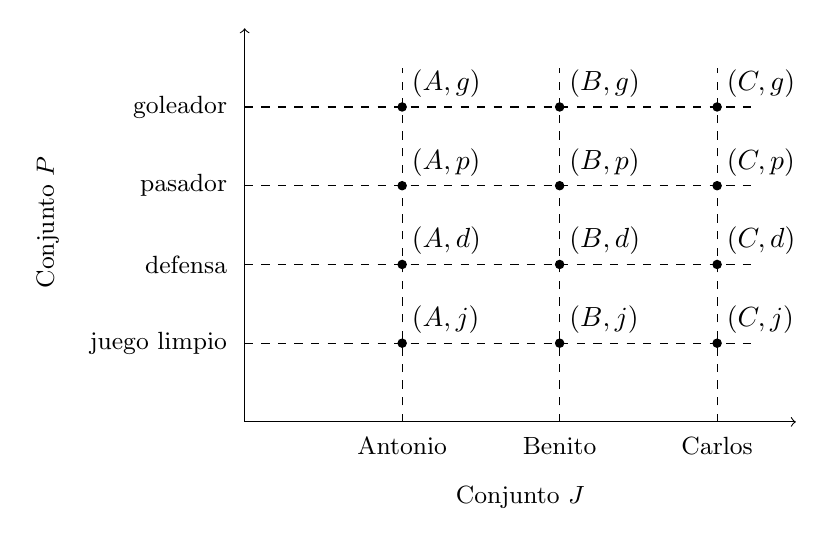
\begin{tikzpicture}[scale=1]
      % Ejes
      \draw[->] (0,0) -- (7,0);
      \draw[->] (0,0) -- (0,5);

      % Etiquetas de los ejes
      \node[left, rotate=90] at (-2.5, 3.5) {\small Conjunto $P$};
      \node[below] at (3.5, -0.7) {\small Conjunto $J$};

      % Etiquetas en los ejes
      \node at (2, -0.3) {\small Antonio};
      \node at (4, -0.3) {\small Benito};
      \node at (6, -0.3) {\small Carlos};

      \node[left] at (-0.1, 1) {\small juego limpio};
      \node[left] at (-0.1, 2) {\small defensa};
      \node[left] at (-0.1, 3) {\small pasador};
      \node[left] at (-0.1, 4) {\small goleador};

      % Líneas punteadas horizontales
      \foreach \y in {1,2,3,4} {
          \draw[dashed] (0,\y) -- (6.5,\y);
      }

      % Líneas punteadas verticales
      \foreach \x in {2,4,6} {
          \draw[dashed] (\x,0) -- (\x,4.5);
      }

      % Puntos y etiquetas
      \filldraw (2,1) circle (1.5pt) node[anchor=south west] {$(A, j)$};
      \filldraw (4,1) circle (1.5pt) node[anchor=south west] {$(B, j)$};
      \filldraw (6,1) circle (1.5pt) node[anchor=south west] {$(C, j)$};

      \filldraw (2,2) circle (1.5pt) node[anchor=south west] {$(A, d)$};
      \filldraw (4,2) circle (1.5pt) node[anchor=south west] {$(B, d)$};
      \filldraw (6,2) circle (1.5pt) node[anchor=south west] {$(C, d)$};

      \filldraw (2,3) circle (1.5pt) node[anchor=south west] {$(A, p)$};
      \filldraw (4,3) circle (1.5pt) node[anchor=south west] {$(B, p)$};
      \filldraw (6,3) circle (1.5pt) node[anchor=south west] {$(C, p)$};

      \filldraw (2,4) circle (1.5pt) node[anchor=south west] {$(A, g)$};
      \filldraw (4,4) circle (1.5pt) node[anchor=south west] {$(B, g)$};
      \filldraw (6,4) circle (1.5pt) node[anchor=south west] {$(C, g)$};
    \end{tikzpicture}
    }
    \caption{Representación cartesiana del conjunto $J \times P$}
    \label{fig:conjunto_cartesiano}
  \end{figure}
\end{example}





\subsection{Propiedades}

El producto de conjuntos tiene las propiedades siguientes, de las que, a
modo de ejercicio, demostraremos una de ellas. Cualesquiera que sean los
conjuntos $A$, $A'$, $B$, $B'$ y $C$, se cumple:

\begin{enumerate}
  \item Si $A' \subseteq A$ y $B' \subseteq B$, entonces $A' \times B'
    \subseteq A \times B$.

  \item Propiedad distributiva del producto respecto a la unión.

  \begin{align*}
    (A \cup B) \times C &= (A \times C) \cup (B \times C) \\
    A \times (B \cup C) &= (A \times B) \cup (A \times C) \\
  \end{align*}

\item Propiedad distributiva del producto respecto a la intersección.

  \begin{align*}
    (A \cap B) \times C &= (A \times C) \cap (B \times C) \\
    A \times (B \cap C) &= (A \times B) \cap (A \times C) \\
  \end{align*}

  \item $A \times B = \emptyset$ si y solo si $A = \emptyset$ o $B =
    \emptyset$.
\end{enumerate}

\begin{exercise}
  Demuestre la propiedad distributiva siguiente:

  \[ A \times (B \cap C) = (A \times B) \cap (A \times C) \]

  Demostramos las dos inclusiones

  \begin{align*}
    A \times (B \cap C) \subseteq (A \times B) \cap (A \times C) \\
    A \times (B \cap C) \supseteq (A \times B) \cap (A \times C) \\
  \end{align*}

  Sea $(x, y)$ un elemento arbitrario de $A \times (B \cap C)$. En
  consecuencia, $x \in A$ e $y \in B \cap C$. Luego $y$ es elemento de $B$ y
  de $C$, por lo que $(x, y) \in A \times B$ y $(x, y) \in A \times C$. Por
  tanto, $(x, y) \in (A \times B) \cap (A \times C)$.

  Inversamente, son cualquier par $(x, y) \in (A \times B) \cap (A \times
  C)$. Por tanto, $(x, y) \in A \times B$ y $(x, y) \in A \times C$. Es
  decir, $x \in A$ e $y \in B$ y, además, $x \in A$ e $y \in C$. Como $y$ es
  elemento de ambos conjuntos $B$ y $C$, resulta que $y \in B \cap C$. En
  consecuencia, $(x, y) \in A \times (B \cap C)$.
\end{exercise}

El producto de conjuntos distintos no cumple la propiedad conmutativa. Es
decir, dados dos conjuntos $A$ y $B$, en general se tiene que

\[ A \times B \neq B \times A \]

El concepto de producto de dos conjuntos se puede ampliar a producto de tres
o más conjuntos.

Dados un elemento $x$ de un conjunto $A$, $x \in A$, un elemento $y$ de otro
conjunto $B$, $y \in B$, y otro elemento $z$ de un tercer conjunto $C$, $z
\in C$, existen seis posibles ordenaciones de los tres elementos. Cada
ordenación se denomina \semph{terna ordenada} (\emph{ordered triples}) y se
escriben como $(x, y, z)$, $(x, z, y)$, $(y, x, z)$, $(y, z, x)$, $(z, x,
y)$ y $(z, y, x)$.

Dos ternas $(x, y, z)$ y $(p, q, r)$ son iguales si y solo si $x = p$, $y =
q$ y $z = r$.

Dados tres conjuntos $A$, $B$ y $C$, se denomina producto (o producto
cartesiano) de $A$ por $B$ y $C$ al conjunto de ternas ordenadas

\[ A \times B \times C = \{(x, y, z) \st x \in A, \quad y \in B \quad
\text{y} \quad z \in C\} \]

Si $A = B = C$, se escribe $A^3$ en lugar de $A \times A \times A$.

Este mismo concepto, además de a 3 conjuntos se puede generalizar a un
número arbitrario (entero positivo, evidentemente) de conjuntos.

Dados $n$ conjuntos $A_1, A_2, A_3, \ldots, A_n$, se denomina ``producto de
$A_1$ por $A_2$ por $A_3$ \dots{} por $A_n$'' al conjunto

\[ A_1 \times A_2 \times \cdots \times A_n = \{(x_1, x_2, \ldots, x_n) \st
x_1 \in A_1, \ x_2 \in A_2, \ \ldots, \ x_n \in A_n\} \]

Los elementos de $A_1 \times A_2 \times \cdots \times A_n$ se llaman
``$n$-tuplas'' (\emph{$n$-tuples}). También hay quien las llama
\emph{listas} (\emph{lists}).\footnotemark

\footnotetext{En combinatoria es bastante común llamarlas \emph{listas}.}

Si $A_1 = A_2 = \cdots = A_n = A$, se escribe $A^n$ en lugar de $A \times A
\times \cdots \times A$.

\begin{example}
  Puntos del espacio tridimensional euclídeo.

  Un punto del espacio euclídeo, dotado de un sistema de referencia,
  representa una terna ordenada de números reales. Por ejemplo, el punto
  $(2, 3, {-2})$. El espacio real completo representa al conjunto $\rset^3 =
  \rset \times \rset \times \rset$. Vea la
  figura~\ref{fig:espacio_euclideo}.

  \begin{figure}
    \centering
    \foreignlanguage{english}{
    \begin{tikzpicture}[scale=1]
      % Dibujar los ejes
      \draw[->] (0, 0, 0) -- (4, 0, 0) node[below right] {$OX$};
      \draw[->] (0, 0, 0) -- (0, 4, 0) node[below left] {$OY$};
      \draw[->] (0, 0, 0) -- (0, 0, 4) node[above left] {$OZ$};

      % Etiquetas de los valores
      \node[above] at (0.8, 0, 0) {$x$};
      \node[below left] at (0, 0.7, 0) {$y$};
      \node[left] at (0, 0, 0.7) {$z$};

      % Coordenadas del punto P
      \coordinate (P) at (1.5, 3.5, 2.5);

      % Proyecciones punteadas del punto P
      \draw[dashed] (1.5, 0, 0) -- (1.5, 0, 2.5) -- (P);
      \draw[dashed] (0, 3.5, 0) -- (P);
      % \draw[dashed] () -- (0, 1.5, 0);

      % Proyección en el plano XY
      % \draw[dashed] (2, 1.5, 0) -- (0, 1.5, 0);

      % Etiqueta del punto P
      \filldraw (P) circle (1.5pt) node[right] {$P = (x, y, z)$};
    \end{tikzpicture}
  }
    \caption{Representación cartesiana del espacio euclídeo}
    \label{fig:espacio_euclideo}
  \end{figure}
\end{example}






